\section{The arcs}
\begin{NewMacroBox}{tkzDrawArc}{\oarg{local options}\parg{O,\dots}\parg{\dots}}%

This macro traces the arc of center $O$. Depending on the options, the arguments differ.   It is a question of determining a starting point and an end point. Either the starting point is given, which is the simplest, or the radius of the arc is given. In the latter case, it is necessary to have two angles. Either the angles can be given directly, or nodes associated with the center can be given to determine them. The angles are in degrees.

\medskip

\begin{tabular}{lll}%
\toprule
options             & default & definition                        \\
\midrule
\TOline{towards}{towards}{$O$ is the center and the arc from $A$ to $(OB)$}
\TOline{rotate} {towards}{the arc starts from $A$ and the angle determines its length}
\TOline{R}{towards}{We give the radius and two angles}
\TOline{R with nodes}{towards}{We give the radius and two points}
\TOline{angles}{towards}{We give the radius and two points}
\TOline{delta}{0}{angle added on each side }
\bottomrule
\end{tabular}

\medskip
Of course, you have to add all the styles of \TIKZ\ for the tracings...

\medskip

\begin{tabular}{lll}%
\toprule
options             & arguments & example                         \\
\midrule
\TOline{towards}{\parg{pt,pt}\parg{pt}}{\tkzcname{tkzDrawArc[delta=10](O,A)(B)}}
\TOline{rotate} {\parg{pt,pt}\parg{an}}{\tkzcname{tkzDrawArc[rotate,color=red](O,A)(90)}}
\TOline{R}{\parg{pt,$r$}\parg{an,an}}{\tkzcname{tkzDrawArc[R](O,2 cm)(30,90)}}
\TOline{R with nodes}{\parg{pt,$r$}\parg{pt,pt}}{\tkzcname{tkzDrawArc[R with nodes](O,2 cm)(A,B)}}
\TOline{angles}{\parg{pt,pt}\parg{an,an}}{\tkzcname{tkzDrawArc[angles](O,A)(0,90)}}
\end{tabular}
\end{NewMacroBox}

Here are a few examples:

\subsection{Option \tkzname{towards}}
It's useless to put \tkzname{towards}. In this first example the arc starts from $A$ and goes to $B$. The arc going from $B$ to $A$ is different. The salient is obtained by going in the direct direction of the trigonometric circle.
\begin{tkzexample}[latex=6cm,small]
\begin{tikzpicture}
  \tkzDefPoint(0,0){O}
  \tkzDefPoint(2,-1){A}
  \tkzDefPointBy[rotation= center O angle 90](A)
  \tkzGetPoint{B}
  \tkzDrawArc[color=blue,<->](O,A)(B)
  \tkzDrawArc(O,B)(A)
  \tkzDrawLines[add = 0 and .5](O,A O,B)
  \tkzDrawPoints(O,A,B)
  \tkzLabelPoints[below](O,A,B)
\end{tikzpicture}
\end{tkzexample}


\subsection{Option \tkzname{towards}}
In this one, the arc starts from A but stops on the right (OB).

\begin{tkzexample}[latex=6cm,small]
\begin{tikzpicture}[scale=1.5]
  \tkzDefPoint(0,0){O}
  \tkzDefPoint(2,-1){A}
  \tkzDefPoint(1,1){B}
  \tkzDrawArc[color=blue,->](O,A)(B)
  \tkzDrawArc[color=gray](O,B)(A)
  \tkzDrawArc(O,B)(A)
  \tkzDrawLines[add = 0 and .5](O,A O,B)
  \tkzDrawPoints(O,A,B)
  \tkzLabelPoints[below](O,A,B)
\end{tikzpicture}
\end{tkzexample}

\subsection{Option \tkzname{rotate}}
\begin{tkzexample}[latex=5cm,small]
\begin{tikzpicture}
  \tkzDefPoint(0,0){O}
  \tkzDefPoint(2,-2){A}
  \tkzDefPoint(60:2){B}
  \tkzDrawLines[add = 0 and .5](O,A O,B)
  \tkzDrawArc[rotate,color=red](O,A)(180)
  \tkzDrawPoints(O,A,B)
  \tkzLabelPoints[below](O,A,B)
\end{tikzpicture}
\end{tkzexample}


\subsection{Option \tkzname{R}}
\begin{tkzexample}[latex=5cm,small]
\begin{tikzpicture}
  \tkzDefPoints{0/0/O}
  \tikzset{compass style/.append style={<->}}
  \tkzDrawArc[R,color=orange,double](O,3cm)(270,360)
  \tkzDrawArc[R,color=blue,double](O,2cm)(0,270)
  \tkzDrawPoint(O)
  \tkzLabelPoint[below](O){$O$}
\end{tikzpicture}
\end{tkzexample}

\subsection{Option \tkzname{R with nodes}}
\begin{tkzexample}[latex=5cm,small]
\begin{tikzpicture}
  \tkzDefPoint(0,0){O}
  \tkzDefPoint(2,-1){A}
  \tkzDefPoint(1,1){B}
  \tkzCalcLength(B,A)\tkzGetLength{radius}
  \tkzDrawArc[R with nodes](B,\radius pt)(A,O)
\end{tikzpicture}
\end{tkzexample}

\subsection{Option \tkzname{delta}}
This option allows a bit like \tkzcname{tkzCompass} to place an arc and overflow on either side. delta is a measure in degrees.

\begin{tkzexample}[latex=7cm,small]
\begin{tikzpicture}
 \tkzDefPoint(0,0){A}
 \tkzDefPoint(5,0){B}
 \tkzDefPointBy[rotation= center A angle 60](B)
 \tkzGetPoint{C}
 \tkzSetUpLine[color=gray]
 \tkzDefPointBy[symmetry= center C](A)
 \tkzGetPoint{D}
 \tkzDrawSegments(A,B A,D)
 \tkzDrawLine(B,D)
 \tkzSetUpCompass[color=orange]
 \tkzDrawArc[orange,delta=10](A,B)(C)
 \tkzDrawArc[orange,delta=10](B,C)(A)
 \tkzDrawArc[orange,delta=10](C,D)(D)
 \tkzDrawPoints(A,B,C,D)
 \tkzLabelPoints(A,B,C,D)
 \tkzMarkRightAngle(D,B,A)
\end{tikzpicture}
\end{tkzexample}

\subsection{Option \tkzname{angles}: example 1}

\begin{tkzexample}[latex=7cm,small]
\begin{tikzpicture}[scale=.75]
  \tkzDefPoint(0,0){A}
  \tkzDefPoint(5,0){B}
  \tkzDefPoint(2.5,0){O}
  \tkzDefPointBy[rotation=center O angle 60](B)
  \tkzGetPoint{D}
  \tkzDefPointBy[symmetry=center D](O)
  \tkzGetPoint{E}
  \tkzSetUpLine[color=Maroon]
  \tkzDrawArc[angles](O,B)(0,180)
  \tkzDrawArc[angles,](B,O)(100,180)
  \tkzCompass[delta=20](D,E)
  \tkzDrawLines(A,B O,E B,E)
  \tkzDrawPoints(A,B,O,D,E)
  \tkzLabelPoints(A,B,O,D,E)
  \tkzMarkRightAngle(O,B,E)
\end{tikzpicture}
\end{tkzexample}

\subsection{Option \tkzname{angles}: example 2}


\begin{tkzexample}[latex=7cm,small]
  \begin{tikzpicture}
   \tkzDefPoint(0,0){O}
   \tkzDefPoint(5,0){I}
   \tkzDefPoint(0,5){J}
   \tkzInterCC(O,I)(I,O)\tkzGetPoints{B}{C}
   \tkzInterCC(O,I)(J,O)\tkzGetPoints{D}{A}
   \tkzInterCC(I,O)(J,O)\tkzGetPoints{L}{K}
   \tkzDrawArc[angles](O,I)(0,90)
   \tkzDrawArc[angles,color=gray,style=dashed](I,O)(90,180)
   \tkzDrawArc[angles,color=gray,style=dashed](J,O)(-90,0)
   \tkzDrawPoints(A,B,K)
   \foreach \point in {I,A,B,J,K}{\tkzDrawSegment(O,\point)}
  \end{tikzpicture}
\end{tkzexample}


 \endinput

